% Preprint source for paper/NOTE.md.  Build: see paper/latex/README.md.
% Every number below is regenerated by scripts/run_robustness_grid.py and
% scripts/analyze_robustness.py (results/robustness/analysis/).
\documentclass[11pt]{article}

\usepackage[T1]{fontenc}
\usepackage[utf8]{inputenc}
\usepackage{lmodern}
\usepackage[margin=1in]{geometry}
\usepackage{amsmath,amssymb}
\usepackage{graphicx}
\usepackage{booktabs}
\usepackage{array}
\usepackage{caption}
\usepackage[numbers,sort&compress]{natbib}
\usepackage{xcolor}
\usepackage{xurl}
\usepackage[colorlinks=true,linkcolor=blue!50!black,citecolor=blue!50!black,urlcolor=blue!50!black]{hyperref}

% Figures are read straight from the repository so the PDF cannot drift from
% the analysis.  For an arXiv upload, run make_arxiv_bundle.sh, which copies
% them next to this file.
\graphicspath{{figures/}{../../results/robustness/figures/}}

\newcommand{\Mp}[1]{M_{#1}}
\newcommand{\ci}[2]{[#1,\,#2]}

\title{The density advantage in FORCE-trained motor RNNs disappears under a
matched plasticity budget}

\author{%
  Thomas Chisica\\
  \small Universidad del Rosario, Bogot\'a, Colombia
  % ---------------------------------------------------------------------
  % TEAMMATE AUTHORS: PENDING WRITTEN CONSENT.  Do not uncomment until each
  % person has agreed in writing to authorship, author order, affiliation and
  % this text (see CHECKLIST-RELEASE.md).  Until then they are thanked in the
  % Acknowledgements instead.
  % \and
  % [Full name] (GitHub @paulovictormourao)\\ \small [Affiliation]
  % \and
  % [Full name] (GitHub @Keshi)\\ \small [Affiliation]
  % \and
  % [Full name] (GitHub @ferorizarmas)\\ \small [Affiliation]
  % ---------------------------------------------------------------------
}

\date{Preprint, not peer reviewed. \today}

\begin{document}
\maketitle

\begin{abstract}
We studied rate recurrent neural networks (RNNs) trained with FORCE-style
recursive least squares (RLS) on six-target centre-out reaching, following
Feulner \& Clopath~\cite{feulner2021neural}. Recurrent connection density was
varied over $p\in\{0.05,0.10,0.20,0.40\}$, with variance-scaled weights and
paired seeds. With all edges trainable, denser networks perform clearly better:
the contrast H1 (sparse NMSE minus mean denser NMSE) is $+0.190$ (seed-bootstrap
95\% CI \ci{0.154}{0.229}), positive in 16/16 network seeds at $N=200$. When
every density receives the same number of trainable edges, the advantage
disappears: the per-seed drop in H1 is $+0.231$ \ci{0.193}{0.267}, positive in
16/16 seeds. This holds up to 200 training trials, under spectral-radius
matching (16/16), at $N=400$ (8/8), at $N=100$ after 200 trials, and when the
budget is a random subset of each dense mask (8/8). An earlier 8-seed analysis
suggested that the sign \emph{reverses} under the equal budget
($-0.090$ \ci{-0.113}{-0.068}). With 16 seeds this residual is about half as
large, and with matched spectral radii it is not distinguishable from zero. A
factorial ablation detects no density component in it, although it cannot
exclude one of the same size; it is more consistent with a cost of the frozen
recurrent input that such a control introduces. In this model the density
advantage tracks the number of trainable recurrent edges, not structural
density.
\end{abstract}

% =========================================================================
\section{Introduction}

Recurrent connectivity in cortex is sparse. Network models of motor learning
usually fix the connection probability: Feulner \&
Clopath~\cite{feulner2021neural} use 10\%. Connectivity constrains the
low-dimensional activity a circuit can express~\cite{warnberg2019perturbing},
and sparse random reservoirs can compute well even with their recurrent
weights frozen~\cite{jaeger2004harnessing}. Recent studies of trained
networks report that sparse, structured connectivity can speed learning:
locality-masked sparse RNNs with an optimal sparsity train faster and more
data-efficiently than fully connected ones on a large cognitive task
battery~\cite{khona2023winning}, and in large recurrent networks with
cortex-like constraints sparse connectivity facilitates time- and
data-efficient learning~\cite{fruengel2025sparse}.

Sparse, variance-scaled random networks keep the overall recurrent input
statistics of dense ones, so one might expect density to matter little once
the weights are rescaled. With a learning rule that updates every existing
edge, such as FORCE/RLS~\cite{sussillo2009generating}, density changes two
things at once: (i) the structure of the recurrent graph, and (ii) the number
of weights the rule can change, which scales as $pN^2$.

Our Neuromatch Academy project first observed that denser networks learned
the reaching task better when every existing edge was trainable. We then asked
whether this survives when the number of trainable edges is held fixed. The
first control suggested a clean sign reversal. This note reports the
robustness checks we ran before trusting that reversal, and what is left of
it.

\paragraph{Contribution.} A small, fully reproducible case study (paired
seeds, held-out evaluation with a fixed decoder, exact identity checks between
arms) showing that
(1) the density advantage in a FORCE-trained motor RNN is a plasticity-budget
effect; and
(2) the apparent reversal under a matched budget is small and not robust to
gain matching. A factorial ablation detects no density component in it; it is
more consistent with a cost of the frozen edges that such a control
necessarily introduces.
We make no claim about biological circuits.

% =========================================================================
\section{Methods}

\subsection{Model and task}

We use the rate RNN of Feulner \& Clopath~\cite{feulner2021neural} as adapted
in the Neuromatch Academy motor-RNN project template.

\paragraph{Dynamics.} $N$ units with state $r$ and rate $z=\tanh(r)$ evolve as
$\tau\dot r=-r+Wz+W_{\text{in}}u$, with $\tau=0.1$\,s, Euler step
$dt=0.01$\,s and 2\,s trials.

\paragraph{Task.} A 0.2\,s one-hot cue $u$ selects one of six centre-out
targets. The network must then produce a constant 2-D velocity (magnitude 0.2)
through a fixed random linear decoder $D$ ($2\times N$, Frobenius norm 0.04).

\paragraph{Learning.} Recurrent weights are trained online with per-neuron
RLS~\cite{sussillo2009generating} ($P_0=I/20$; an update every second time
step after the cue). The decoder error is assigned to neurons through the
pseudo-inverse $D^{+}$. The decoder, the input weights and all RLS
hyper-parameters never change.

\paragraph{Connectivity.} Structural masks are nested: within a seed, edge
$(i,j)$ exists at density $p$ iff $U_{ij}<p$, for one shared uniform matrix
$U$ (no self-connections). Non-zero weights are $W_{ij}=g\,G_{ij}/\sqrt{pN}$,
with $g=1.5$ and one shared Gaussian matrix $G$. All conditions of a seed share
$U$, $G$, $W_{\text{in}}$, $D$, the training target order and initial states,
and the held-out set. The densities are $p\in\{0.05,0.10,0.20,0.40\}$.

\paragraph{Outcome.} Held-out velocity NMSE under the fixed decoder, with
learning switched off, on 30 trials (5 initial states $\times$ 6 targets).
NMSE $=1$ means ``no better than predicting the mean velocity''. Lower is
better.

\paragraph{Training length.} Every network is trained for 200 trials and
evaluated every 10 trials. The first 60 training trials and the held-out set
are drawn exactly as in the original 60-trial runs; trials 61--200 come from a
separate seeded stream. As a result, the trial-60 checkpoint of seeds 0--7
reproduces the original results to within $1.2\times10^{-12}$ (all 224
overlapping checkpoints). The original snapshot is therefore a checkpoint of
these runs, not a separate experiment.

\subsection{Arms}

\begin{table}[ht]
\centering
\small
\caption{Experimental arms. $\Mp{p}$ is the structural mask at density $p$.}
\label{tab:arms}
\begin{tabular}{>{\raggedright}p{0.27\linewidth}>{\raggedright}p{0.33\linewidth}>{\raggedright\arraybackslash}p{0.30\linewidth}}
\toprule
Arm & Trainable recurrent edges & Initial weights\\
\midrule
All edges trainable (primary) & every existing edge ($\approx pN^2$) & $gG/\sqrt{pN}$ on $\Mp{p}$\\
Equal trainable budget (control) & the $p=0.05$ edges $\Mp{0.05}$ in every density & as primary; edges in $\Mp{p}\setminus\Mp{0.05}$ are frozen\\
R2 gain-matched (both of the above) & as the parent arm & parent $W$ $\times$ scalar, so that $\rho(W_p)=\rho(W_{0.05})$ within the seed\\
Equal budget, random subset (B3) & a uniform random subset of $\Mp{p}$ of the same size as $\Mp{0.05}$ (separate random stream) & as primary; the other edges of $\Mp{p}$ are frozen\\
R3 frozen-drive factorial & $\Mp{0.05}$ & see Section~\ref{sec:r3}\\
R3 with unmatched total gain (B4) & $\Mp{0.05}$ & see Section~\ref{sec:r3}\\
\bottomrule
\end{tabular}
\end{table}

Because the masks are nested, the control's trainable \emph{set} is identical
across densities, not just its size. The random-subset arm keeps only the
size: its trainable edges are spread over the dense mask, are not nested
across densities, and start from the smaller dense-network weights
$gG/\sqrt{pN}$. At $p=0.05$ both equal-budget arms are the primary network
(verified identical).

\subsection{R3: separating frozen drive from density}
\label{sec:r3}

In the control, raising $p$ changes three things at once: (1) the number of
frozen edges, which is density itself; (2) the share of recurrent input
variance carried by frozen edges, $f_p=(p-0.05)/p=0$, 0.5, 0.75 or 0.875; and
(3) correspondingly, the size of the trainable weights. To separate the first
from the other two we build, for structural density $p$ and frozen share $f$,
\begin{equation}
W=\frac{g\sqrt{1-f}}{\sqrt{0.05N}}\,G\odot\Mp{0.05}
 +\frac{g\sqrt{f}}{\sqrt{(p-0.05)N}}\,G\odot(\Mp{p}\setminus\Mp{0.05}),
\end{equation}
with only $\Mp{0.05}$ trainable. The expected total recurrent input variance
per unit is $g^2$ in every cell.

\paragraph{Grid.} We run the full factorial
$p\in\{0.10,0.20,0.40\}\times f\in\{0.5,0.75,0.875\}$, plus $f=0$ (identical
for every $p$). Along the \emph{density} axis at fixed $f$, the trainable
sub-network is bit-for-bit identical across $p$ and the frozen drive has the
same variance; the only difference is how many frozen edges carry that
variance. Along the \emph{frozen-share} axis at fixed $p$, the edge set is
identical; the only difference is how much drive is frozen.

\paragraph{Anchors.} The diagonal cells $(0.10,0.5)$, $(0.20,0.75)$ and
$(0.40,0.875)$ are exactly the control networks, and $f=0$ is exactly the
$p=0.05$ network. All four reproduced the control's held-out NMSE exactly in
every seed, so the factorial is anchored to the control rather than being a
new model.

\paragraph{Avoiding a degenerate design.} The obvious alternative, deleting
the frozen edges, makes every network identical to $p=0.05$ and cannot measure
anything. Holding $g^2$ fixed also keeps ``more frozen input'' from being
confounded with ``more total gain''.

\paragraph{Unmatched-gain variant (B4).} With $g^2$ fixed, more frozen drive
also means smaller trainable weights (factor $\sqrt{1-f}$). To separate the
two we also run the same $3\times3$ grid with the trainable weights left at
the $p=0.05$ scale, $g/\sqrt{0.05N}$, and the frozen weights as above. The
total input variance is then $g^2(1+f)$; on the diagonal both edge sets keep
their original scales, and $f=0$ is again the $p=0.05$ network. This variant
fixes the trainable weights but trades the confound for another one: total
gain (initial spectral radius 1.9--2.2 against 1.56) grows with $f$.

\subsection{Contrasts and statistics}

\paragraph{Contrasts.} Per seed,
$H1=\text{NMSE}(0.05)-\tfrac13\sum_{p>0.05}\text{NMSE}(p)$ (positive: denser
is better) and
$H2=[\text{NMSE}(0.05)-\text{NMSE}(0.20)]-[\text{NMSE}(0.20)-\text{NMSE}(0.40)]$
(positive: diminishing returns). The primary-minus-control change is the
per-seed difference of the two arms' H1; it is possible because both arms
share all seed-level randomness. For R3 we compute
$\text{density}_f=\text{NMSE}(p{=}0.10,f)-\text{mean NMSE}(p{=}0.20,0.40;f)$,
$\text{frozen}_p=\text{NMSE}(f{=}0)-\text{mean NMSE}(p;f\ge0.5)$, and per-seed
least-squares slopes of NMSE on $\log_2 p$ and on $f$ over the $3\times3$
factorial.

\paragraph{Inference.} The network seed is the replicate. We report the mean,
a seed-bootstrap 95\% percentile interval of the mean (100\,000 resamples,
fixed generator seed), the number of positive seeds, and an exact two-sided
sign test. The smallest attainable sign-test $p$ is 0.0078 with 8 seeds and
$3.1\times10^{-5}$ with 16. No correction for multiple comparisons is
applied; the intervals are descriptive.

\paragraph{Provenance.} H1 and H2 were first committed together with the
primary results (commit \texttt{3021081}, 14 Jul 2026), so they are
\emph{not} preregistered, although early project documents called them
``confirmatory''. They were fixed before the equal-budget control was run
(\texttt{920ff92}, 29 Aug 2026). The robustness checks R1--R5 were specified
in writing before they were run (9 Oct 2026), in response to an independent
audit. We treat every contrast as exploratory.

\paragraph{Robustness checks.}
R1 (convergence): 200 trials; checkpoints 60, 100, 150 and 200.
R2 (gain matching): initial spectral radius matched to the $p=0.05$ network.
R3 (frozen drive vs density): Section~\ref{sec:r3}.
R4 (network size): $N\in\{100,200,400\}$.
R5 (more seeds): 16 seeds at $N=200$.
A second session (10 Oct 2026) extended R2 and R3 to 16 seeds and added B3,
the random-subset equal budget (8 seeds), and B4, the unmatched-gain R3
variant (8 seeds); these were listed as pending checks in the first session's
record before they were run. Unless stated otherwise, everything uses
$N=200$; R2, R3 and R5 use 16 seeds and the other checks seeds 0--7.

% =========================================================================
\section{Results}

\subsection{With all edges trainable, denser is better, robustly}

\begin{table}[ht]
\centering
\small
\caption{Mean held-out NMSE, $N=200$, 16 seeds.}
\label{tab:nmse}
\begin{tabular}{rcccc}
\toprule
 & \multicolumn{2}{c}{All trainable} & \multicolumn{2}{c}{Equal budget}\\
\cmidrule(lr){2-3}\cmidrule(lr){4-5}
$p$ & trial 60 & trial 200 & trial 60 & trial 200\\
\midrule
0.05 & 0.447 & 0.320 & 0.447 & 0.320\\
0.10 & 0.359 & 0.207 & 0.497 & 0.359\\
0.20 & 0.271 & 0.155 & 0.475 & 0.379\\
0.40 & 0.141 & 0.077 & 0.492 & 0.386\\
\bottomrule
\end{tabular}
\end{table}

With all edges trainable, H1 is positive at every checkpoint and in every
variant at $N=200$, and in every seed except one gain-matched seed
(Table~\ref{tab:nmse}): $+0.190$ \ci{0.154}{0.229} with 16 seeds at trial 60;
$+0.173$ \ci{0.135}{0.210} at trial 200; and $+0.175$ \ci{0.128}{0.218},
positive in 15/16, gain-matched at trial 200.

H2 (diminishing returns) is not supported at the original snapshot: $+0.046$
\ci{-0.018}{0.111}, 9/16. At trial 200 it is weakly positive ($+0.087$
\ci{0.004}{0.170}, 9/16), so we do not treat it as established.

\subsection{Under an equal budget the advantage disappears}

\begin{figure}[ht]
\centering
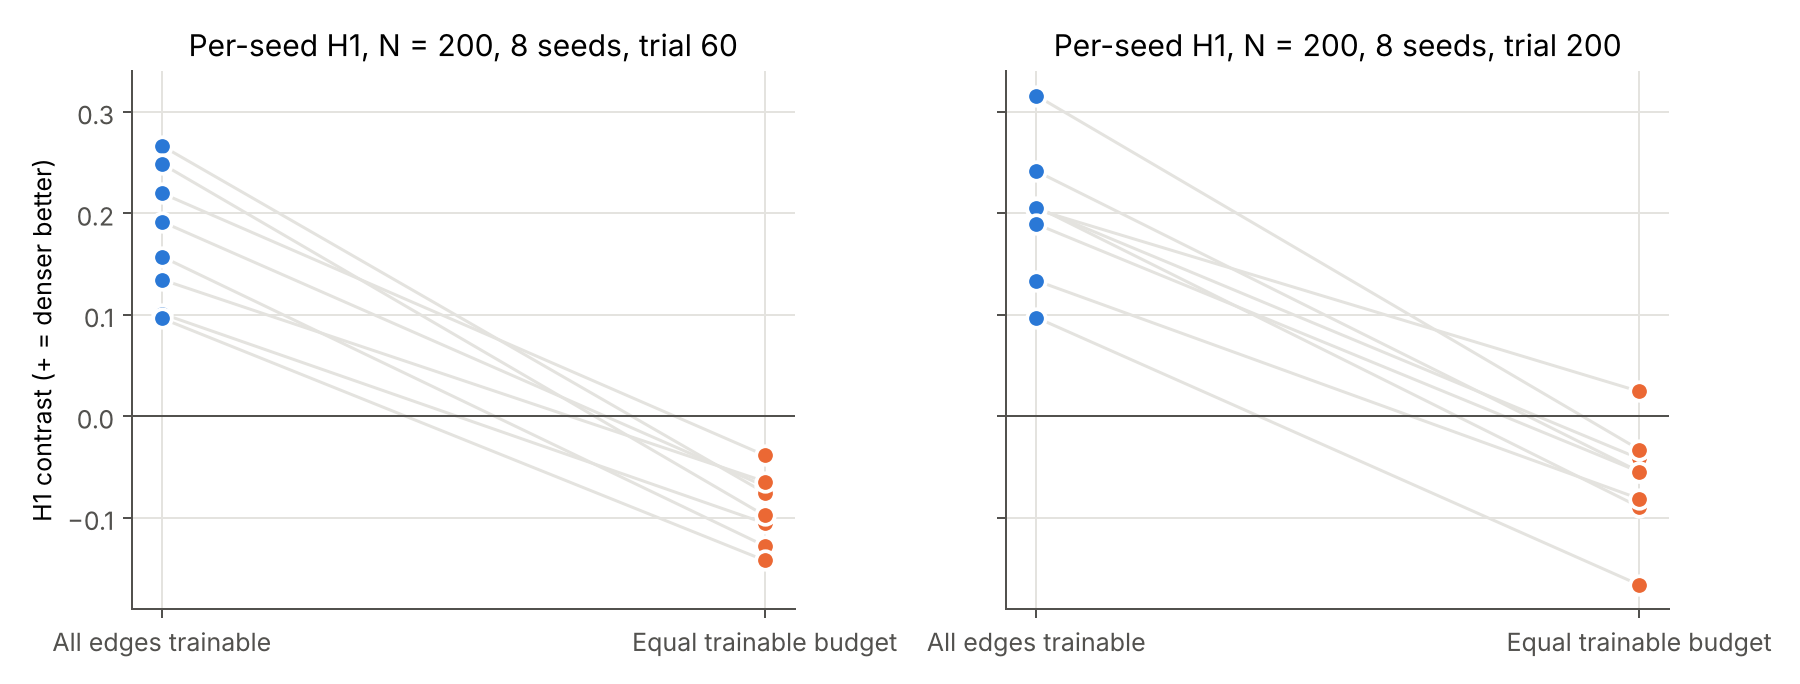
\includegraphics[width=\linewidth]{R5_sixteen_seeds.png}
\caption{Per-seed H1 ($N=200$, 16 seeds) with all edges trainable and under
an equal trainable budget, at trial 60 (left) and trial 200 (right). Lines
join the two arms of the same seed. Positive H1 means denser is better.}
\label{fig:r5}
\end{figure}

The paired primary-minus-control change in H1 is the most robust number in
this study. It is positive in every seed of every check that ran
(Table~\ref{tab:paired}, Figure~\ref{fig:r5}).

\begin{table}[ht]
\centering
\small
\caption{Paired change in H1 (primary $-$ control): mean, 95\% seed-bootstrap
CI, positive seeds.}
\label{tab:paired}
\begin{tabular}{lll}
\toprule
Check & Paired change & Positive\\
\midrule
Original snapshot, 8 seeds, trial 60 & $+0.267$ \ci{0.232}{0.304} & 8/8\\
R1, trial 200 & $+0.261$ \ci{0.228}{0.296} & 8/8\\
R2 gain-matched, 16 seeds, trial 60 & $+0.205$ \ci{0.169}{0.242} & 16/16\\
R2 gain-matched, 16 seeds, trial 200 & $+0.214$ \ci{0.184}{0.249} & 16/16\\
B3 random-subset budget, trial 60 & $+0.246$ \ci{0.170}{0.317} & 8/8\\
B3 random-subset budget, trial 200 & $+0.248$ \ci{0.207}{0.285} & 8/8\\
R5, 16 seeds, trial 60 & $+0.231$ \ci{0.193}{0.267} & 16/16 ($p=3\times10^{-5}$)\\
R5, 16 seeds, trial 200 & $+0.229$ \ci{0.191}{0.265} & 16/16\\
R4, $N=100$, trial 200 & $+0.179$ \ci{0.096}{0.273} & 8/8\\
R4, $N=400$, trial 200 & $+0.069$ \ci{0.060}{0.079} & 8/8\\
\bottomrule
\end{tabular}
\end{table}

The denser networks' advantage therefore depends on their extra trainable
edges. Holding the number of trainable edges fixed removes all of it, whether
the trainable edges are the sparse network's edges or a random subset of the
dense mask (Figure~\ref{fig:b3}).

\begin{figure}[ht]
\centering
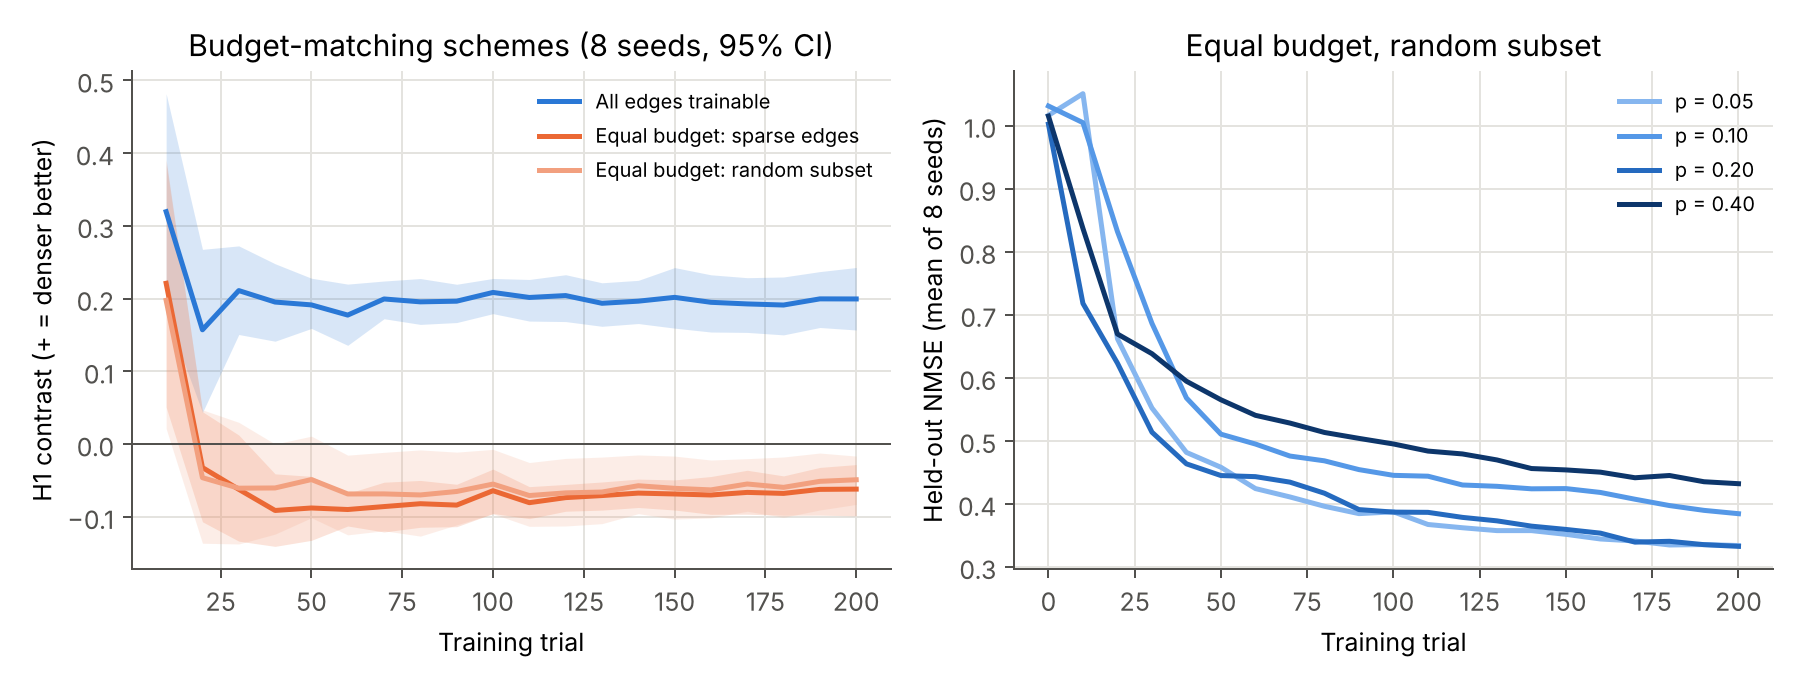
\includegraphics[width=\linewidth]{B3_random_subset.png}
\caption{Budget-matching schemes (8 seeds). Left: H1 over training with all
edges trainable, with the equal budget formed by the sparse network's edges,
and with the equal budget formed by a random subset of each dense mask (B3);
shaded bands are 95\% seed-bootstrap CIs. Right: mean held-out NMSE per
density in the random-subset arm.}
\label{fig:b3}
\end{figure}

\subsection{The sign reversal is small and fragile}

\begin{table}[ht]
\centering
\small
\caption{Equal-budget H1 in each check (negative = sparse better).}
\label{tab:reversal}
\begin{tabular}{lll}
\toprule
Check & Equal-budget H1 & Negative seeds\\
\midrule
Original 8 seeds, trial 60 & $-0.090$ \ci{-0.113}{-0.068} & 8/8\\
R1, trial 100 / 150 / 200 & $-0.064$ / $-0.069$ / $-0.062$, all CIs $<0$ & 7/8, 8/8, 7/8\\
R2 gain-matched, 8 seeds, trial 60 & $-0.068$ \ci{-0.117}{-0.024} & 8/8\\
R2 gain-matched, 8 seeds, trial 200 & $-0.045$ \ci{-0.108}{+0.009} & 5/8\\
R2 gain-matched, 16 seeds, trial 60 & $-0.027$ \ci{-0.073}{+0.019} & 10/16\\
R2 gain-matched, 16 seeds, trial 200 & $-0.039$ \ci{-0.086}{+0.004} & 9/16\\
B3 random-subset budget, trial 60 & $-0.069$ \ci{-0.125}{-0.015} & 6/8\\
B3 random-subset budget, trial 200 & $-0.049$ \ci{-0.083}{-0.017} & 6/8\\
R5, 16 seeds, trial 60 & $-0.041$ \ci{-0.083}{+0.011} & 13/16\\
R5, 16 seeds, trial 200 & $-0.055$ \ci{-0.100}{-0.011} & 12/16\\
R4, $N=100$, trial 200 & $-0.084$ \ci{-0.142}{-0.023} & 6/8\\
R4, $N=400$, trial 200 & $-0.014$ \ci{-0.027}{-0.002} & 6/8\\
\bottomrule
\end{tabular}
\end{table}

The point estimate is negative in every check (Table~\ref{tab:reversal}), but
the effect is small and fragile. Its magnitude roughly halves when the seed
count doubles: seeds 8--15 alone average $+0.008$ at trial 60 ($-0.049$ at
trial 200), so the original 8-seed estimate was optimistic. Under gain
matching with 16 seeds the interval includes zero at both checkpoints, and
only 9--10 of 16 seeds are negative. The random-subset budget (B3) gives a
negative H1 at 8 seeds, but so did the original control at 8 seeds before it
halved. ``Denser is worse under an equal budget'' is therefore at most a
modest tendency, not a clean reversal. We do not claim it.

\paragraph{Spectral radius.} The initial spectral radius was not controlled
in the original runs (1.48--1.65). In seeds 0--7 the sparse-minus-denser
radius gap correlated with primary H1 at $r=-0.90$. Over 16 seeds this falls
to $r=-0.26$ (primary) and $r=+0.20$ (control). Matching the radii (R2)
leaves both the primary advantage and the paired change intact
(Figure~\ref{fig:r2}). The strong correlation was a small-sample coincidence,
not a mechanism.

\begin{figure}[ht]
\centering
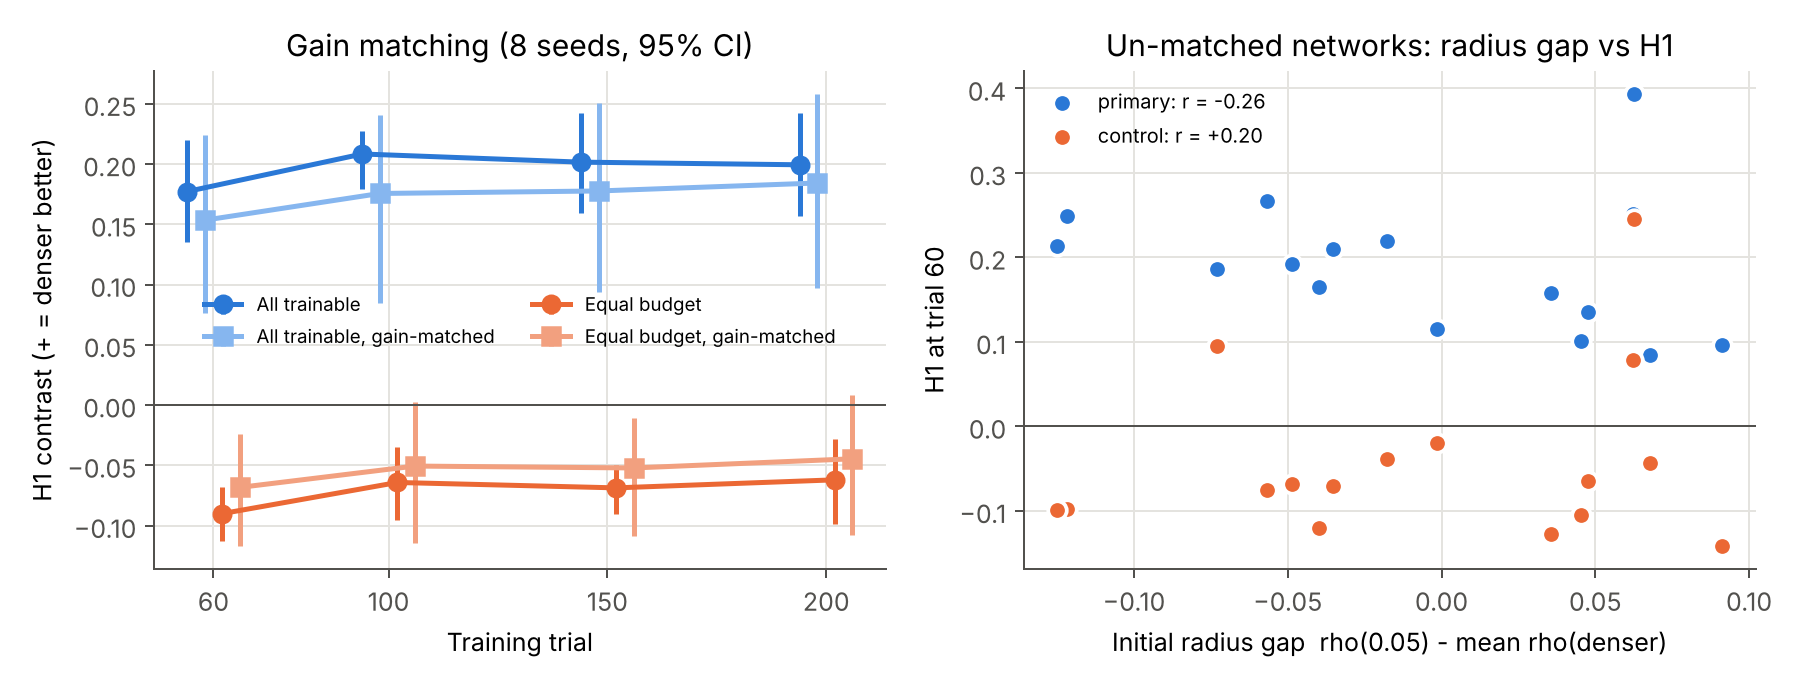
\includegraphics[width=\linewidth]{R2_gain_matched.png}
\caption{Gain matching (16 seeds). Left: H1 at each checkpoint with and
without initial spectral-radius matching (95\% CIs). Right: in the unmatched
networks, the initial radius gap $\rho(0.05)-$ mean $\rho$(denser) against H1
at trial 60.}
\label{fig:r2}
\end{figure}

\subsection{Convergence}

\begin{figure}[ht]
\centering
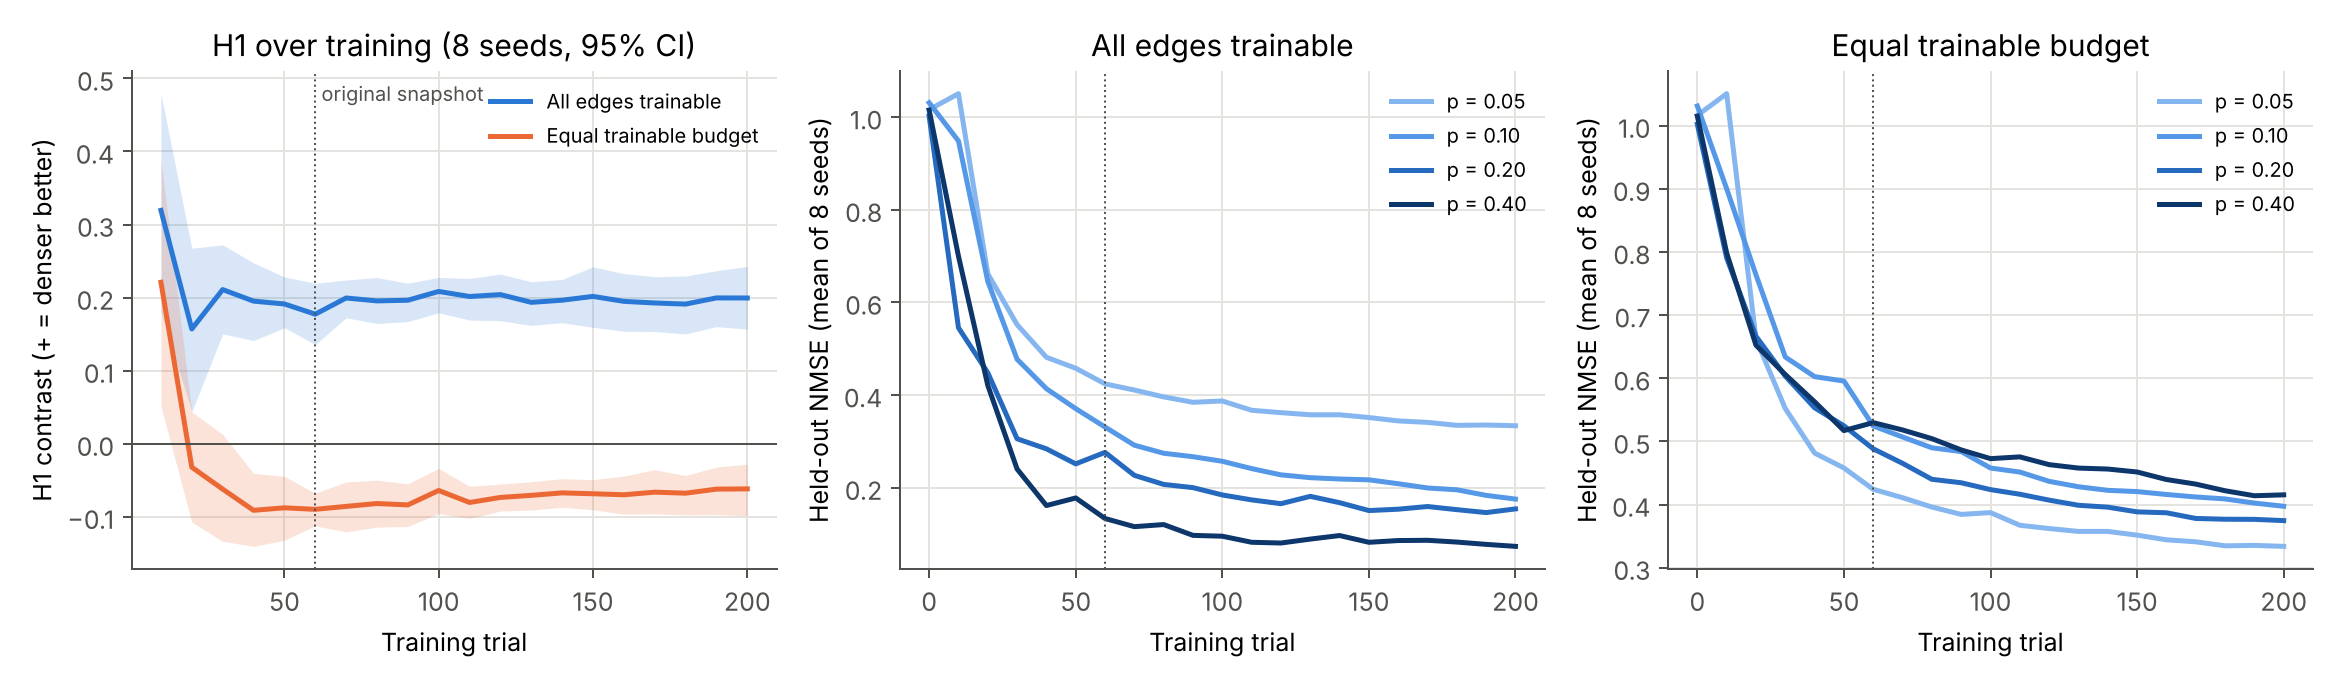
\includegraphics[width=\linewidth]{R1_convergence.png}
\caption{Convergence (8 seeds). Left: H1 over 200 training trials for both
arms (95\% CIs); the dotted line marks the original trial-60 snapshot.
Middle and right: mean held-out NMSE per density in each arm.}
\label{fig:r1}
\end{figure}

The original trial-60 snapshot was taken mid-learning: 23/32 primary networks
were still improving between trials 50 and 60. Training to 200 trials lowers
every NMSE substantially, but every contrast stays within its trial-60
interval (Figure~\ref{fig:r1}): primary H1 goes from $+0.177$ to $+0.199$
\ci{0.157}{0.243}; control H1 from $-0.090$ to $-0.062$ \ci{-0.099}{-0.028};
and the paired change from $+0.267$ to $+0.261$.

The networks are still not fully converged at 200 trials. Between trials 150
and 200, 23/32 primary and 26/32 control networks improved (median relative
NMSE change $-11\%$ and $-7\%$). Between trials 190 and 200 only about half
improved (17/32 and 15/32), which is consistent with a plateau plus noise. H1
was flat from trial 40 onward in both arms.

\subsection{No density component is detected in the control's residual tendency}

\begin{figure}[ht]
\centering
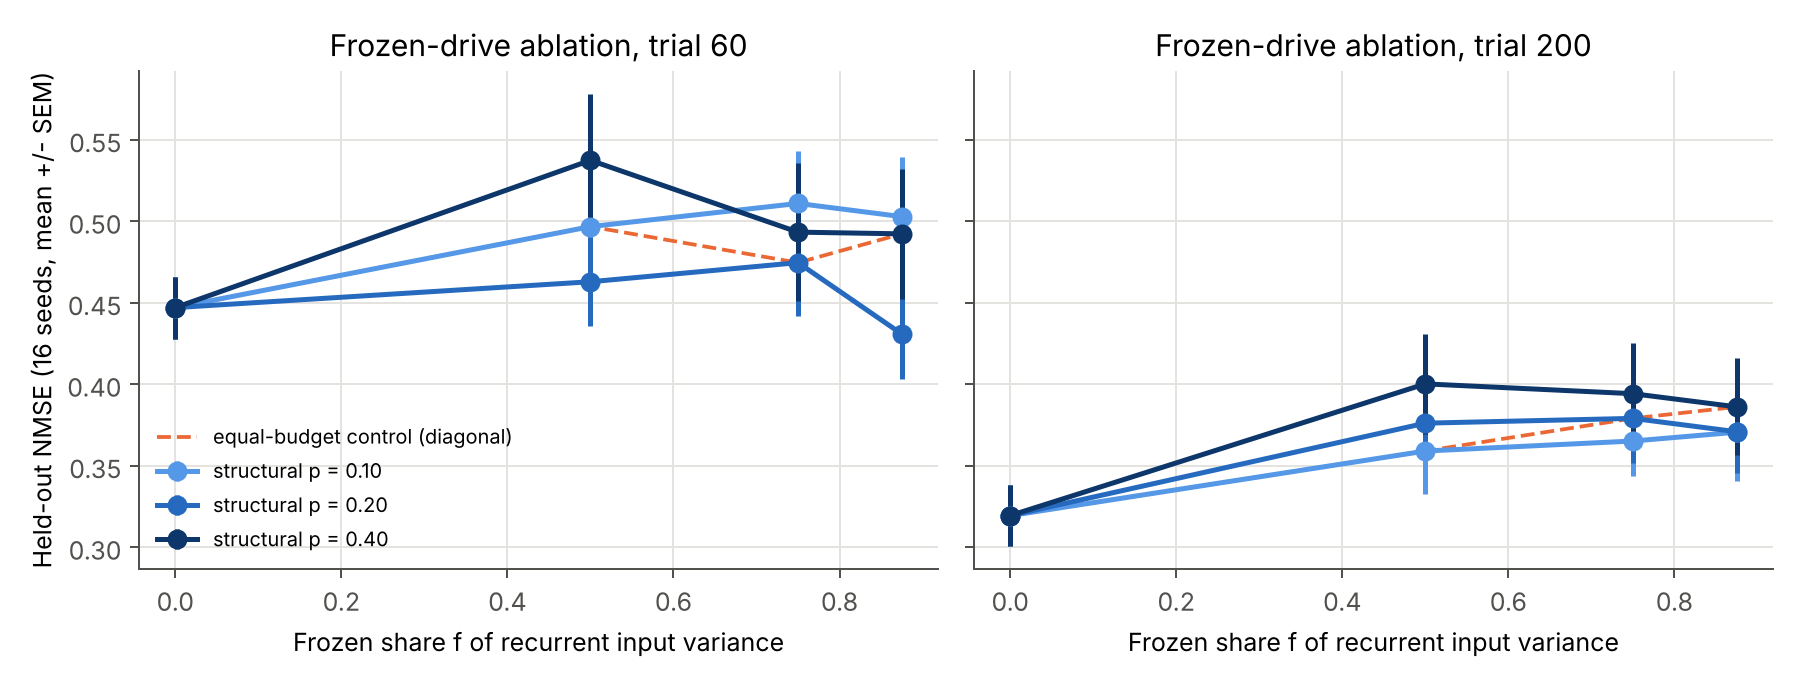
\includegraphics[width=\linewidth]{R3_frozen_drive.png}
\caption{Frozen-drive ablation R3 (16 seeds, mean $\pm$ SEM), at trial 60
(left) and trial 200 (right). Each line is one structural density; the
dashed line joins the diagonal cells, which are exactly the equal-budget
control networks.}
\label{fig:r3}
\end{figure}

\paragraph{Density at a fixed frozen share has no detectable effect} (R3, 16
seeds; Table~\ref{tab:r3density}, Figure~\ref{fig:r3}).

\begin{table}[ht]
\centering
\small
\caption{R3 density contrasts (16 seeds).}
\label{tab:r3density}
\begin{tabular}{lll}
\toprule
R3 contrast & Trial 60 & Trial 200\\
\midrule
density, $f=0.5$ & $-0.003$ \ci{-0.069}{0.062} & $-0.029$ \ci{-0.093}{0.042}\\
density, $f=0.75$ & $+0.027$ \ci{-0.049}{0.104} & $-0.021$ \ci{-0.077}{0.034}\\
density, $f=0.875$ & $+0.041$ \ci{-0.038}{0.121} & $-0.008$ \ci{-0.078}{0.065}\\
slope per doubling of $p$ & $+0.002$ \ci{-0.037}{0.043} & $+0.014$ \ci{-0.018}{0.047}\\
\bottomrule
\end{tabular}
\end{table}

All intervals include zero and are centred near it; the 16-seed slope
intervals are about half as wide as the 8-seed ones. This is the most solid
part of the R3 result, but it is an absence of evidence, not evidence of
absence. The trial-200 density contrasts reach $-0.08$ to $-0.09$, and the
slope's upper bound ($+0.047$ per doubling, two doublings from $p=0.10$ to
$0.40$) allows up to $\approx0.09$ NMSE. Both exceed the control's reversal
($-0.055$), so a density component of that size cannot be excluded. Excluding
it would need intervals of about $\pm0.03$, i.e.\ roughly four times as many
seeds.

\paragraph{Adding frozen drive at a fixed density: a small cost, clear only
at trial 200} (Table~\ref{tab:r3frozen}).

\begin{table}[ht]
\centering
\small
\caption{R3 frozen-drive contrast: NMSE($f=0$) minus mean NMSE over
$f\ge0.5$ (16 seeds); positive seeds in parentheses.}
\label{tab:r3frozen}
\begin{tabular}{lll}
\toprule
& Trial 60 & Trial 200\\
\midrule
$p=0.10$ & $-0.056$ \ci{-0.116}{0.003} (6/16) & $-0.045$ \ci{-0.092}{0.001} (6/16)\\
$p=0.20$ & $-0.009$ \ci{-0.067}{0.052} (7/16) & $-0.056$ \ci{-0.110}{-0.001} (5/16)\\
$p=0.40$ & $-0.061$ \ci{-0.124}{0.007} (4/16) & $-0.074$ \ci{-0.129}{-0.022} (4/16)\\
\bottomrule
\end{tabular}
\end{table}

With 8 seeds two of these three intervals excluded zero at trial 60; with 16
seeds none does, and the per-seed sign tests are not significant
($p\ge0.077$). At trial 200 the mean NMSE rises from 0.320 ($f=0$) to
0.36--0.40 for every cell with $f\ge0.5$, and the slope over
$f\in[0.5,0.875]$ is flat ($-0.005$ \ci{-0.058}{0.043}).

\paragraph{What the unmatched-gain variant adds (B4, 8 seeds).} Keeping the
trainable weights at full size and adding frozen drive on top is far worse:
NMSE 0.53--0.72 at trial 200 against 0.334 at $f=0$ (frozen-drive cost
$-0.30$ to $-0.34$, 8/8 seeds in every column), and the cost now grows with
$f$ (slope $+0.350$ \ci{0.273}{0.426} per unit $f$, 8/8;
Figure~\ref{fig:b4}). Every unmatched cell is worse than the matching
gain-matched R3 cell (mean difference $-0.260$ \ci{-0.300}{-0.222}, 8/8). So
shrinking the trainable weights is not what makes R3's frozen-drive cells
worse: at the same frozen drive, full-size trainable weights do worse, not
better. Because the unmatched networks also have larger total gain, B4 cannot
say whether frozen drive as such or the extra gain does the damage; density
again has no effect at fixed $f$ (slope $+0.007$ \ci{-0.024}{0.037}).

\begin{figure}[ht]
\centering
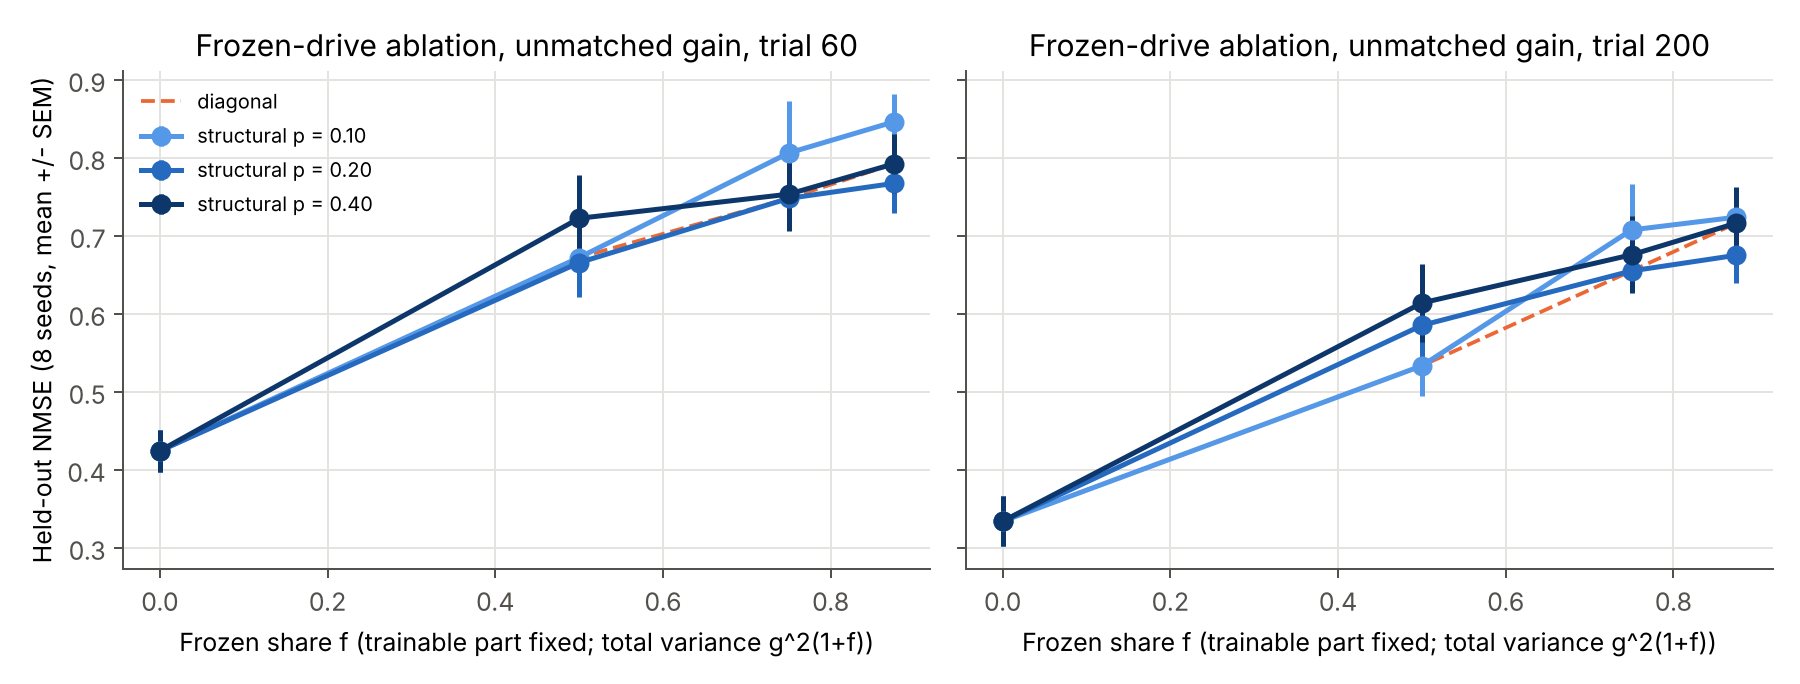
\includegraphics[width=\linewidth]{R3_unmatched_gain.png}
\caption{Frozen-drive ablation with unmatched gain (B4; 8 seeds, mean $\pm$
SEM). The trainable weights keep the $p=0.05$ scale, so total input variance
is $g^2(1+f)$.}
\label{fig:b4}
\end{figure}

\paragraph{Interpretation.} The equal-budget control, rebuilt from the
factorial's diagonal, compares a network with no frozen drive ($p=0.05$)
against three networks that have some. Density at fixed frozen share
contributes nothing detectable, although the ablation is not precise enough
to exclude a density component as large as the control's residual negative
H1. Attributing it to frozen recurrent drive is consistent with the R3 step
at trial 200 and with B4, but the 16-seed evidence for that step is weak
(trial 200 only, sign tests not significant), so we state it as the most
likely explanation rather than as an established result.

\subsection{Network size}

\begin{figure}[ht]
\centering
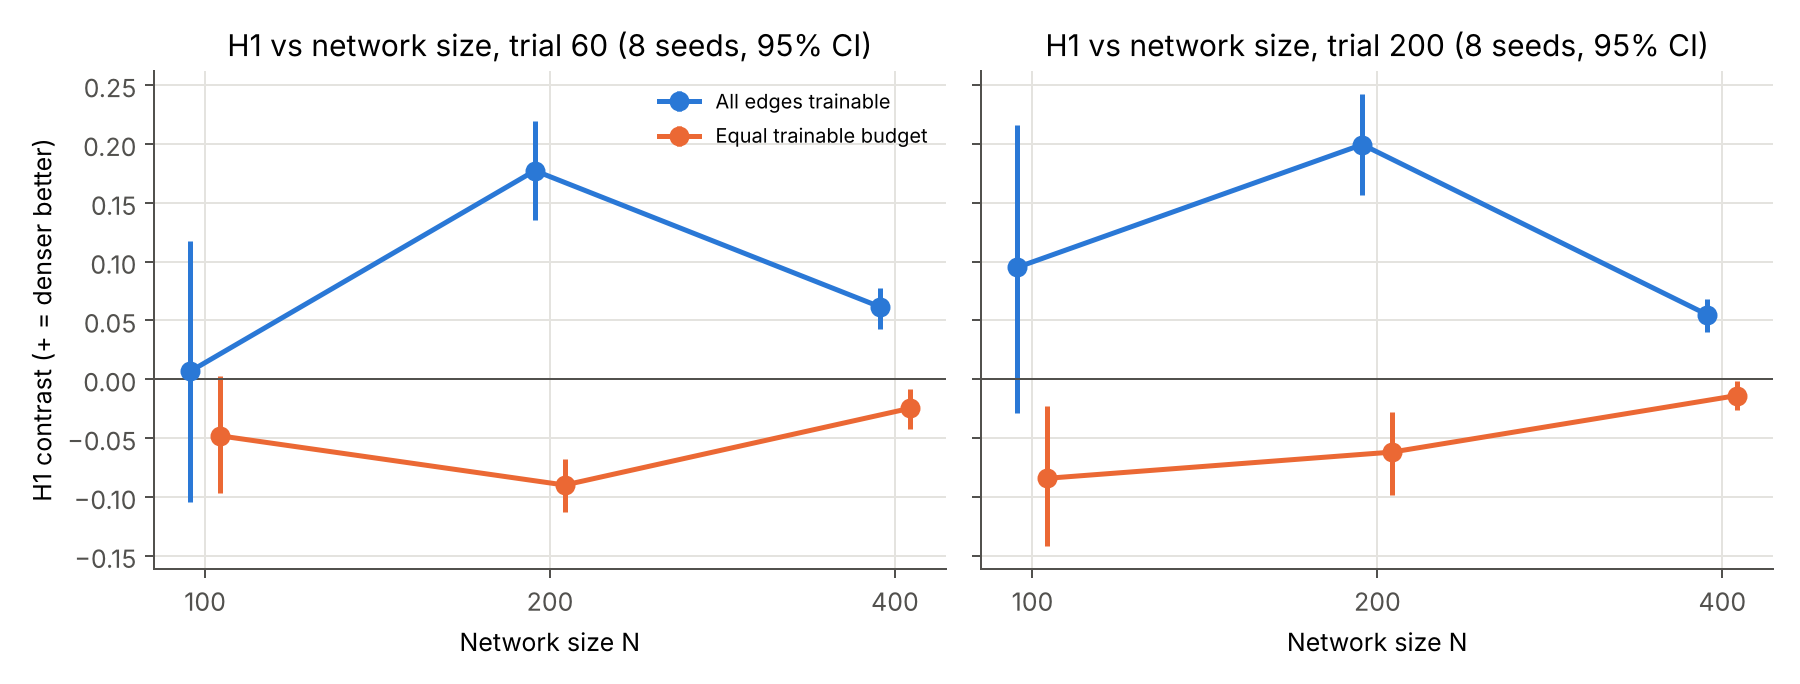
\includegraphics[width=\linewidth]{R4_network_size.png}
\caption{H1 against network size $N$ at trial 60 (left) and trial 200
(right), 8 seeds, 95\% CIs.}
\label{fig:r4}
\end{figure}

\paragraph{$N=100$.} Learning is poor: NMSE 0.60--0.79 at trial 200 and
0.75--0.85 at trial 60, against a chance level of 1. The primary H1 does not
differ from zero (trial 60: $+0.007$ \ci{-0.104}{0.118}; trial 200: $+0.095$
\ci{-0.029}{0.216}). This matches the earlier 3-seed $N=100$ pilot, which had
the opposite sign and which we now read as a regime in which too little is
learned for density to matter. The control H1 is negative at trial 200
($-0.084$ \ci{-0.142}{-0.023}). The paired change is $+0.179$
\ci{0.096}{0.273}, 8/8.

\paragraph{$N=400$.} Learning is much better (trial-200 NMSE 0.012--0.080
with all edges trainable), so every contrast is smaller in absolute NMSE
units. The pattern of $N=200$ is reproduced at both checkpoints
(Figure~\ref{fig:r4}): primary H1 is $+0.062$ \ci{0.043}{0.077} at trial 60
and $+0.055$ \ci{0.040}{0.068} at trial 200, 8/8 positive; equal-budget H1 is
$-0.025$ \ci{-0.042}{-0.008} and $-0.014$ \ci{-0.027}{-0.002}, 6/8 negative;
the paired change is $+0.086$ \ci{0.077}{0.097} and $+0.069$
\ci{0.060}{0.079}, 8/8. In relative terms the effect is large. With all edges
trainable, $p=0.40$ reaches 15\% of the $p=0.05$ NMSE (0.012 vs 0.080). Under
the equal budget, $p=0.05$ is still the best condition (0.080 vs
0.084--0.103).

\paragraph{Across sizes.} The sign pattern holds wherever the networks learn.
Absolute H1 is not comparable across $N$, because the NMSE floor differs.

% =========================================================================
\section{Limitations}

\begin{itemize}
\item \textbf{One model family and one task.} Rate units with tanh,
FORCE/RLS on recurrent weights, a fixed random decoder, and six-target
reaching with constant velocities. We do not test other learning rules
(BPTT, node perturbation), output training, or structured connectivity, so
our results do not speak directly to the sparse-advantage findings obtained
with other architectures and training
procedures~\cite{khona2023winning,fruengel2025sparse}.
\item \textbf{Small samples.} 16 seeds for R2, R3 and R5; 8 seeds for R1, R4,
B3 and B4. R5 and R2 show that 8-seed effect sizes in this system can shrink
by half; the $N=400$, random-subset and unmatched-gain results rest on 8
seeds.
\item \textbf{Not fully converged.} At 200 trials, roughly half of the
networks still improve over the last 10 trials. Contrasts were stable from
trial $\sim$40 onward, but asymptotic behaviour is not established.
\item \textbf{Budget-matching schemes.} We tested two: the sparse network's
edges and a random subset of each dense mask (8 seeds). Both remove the
advantage. Other schemes, such as an equal number of trainable weights per
neuron, were not tested.
\item \textbf{Frozen drive vs gain.} R3 holds total variance at $g^2$, so
more frozen drive also means smaller trainable weights; B4 keeps the
trainable weights fixed but lets total gain grow. Together they rule out
``smaller trainable weights'' as the source of R3's cost, but they do not
separate frozen drive from total gain. The missing cell is shrunken trainable
weights with the frozen edges deleted.
\item \textbf{Gain matching rescales all weights.} It matches the spectral
radius but changes the trainable weights' scale too.
\item \textbf{No population-geometry analysis.} We report task error only.
In a six-target task the dimensionality of population activity is likely to
be bounded by task complexity rather than by the circuit~\cite{gao2017theory},
so we do not interpret manifold dimension here.
\item \textbf{Analysis choices.} H1/H2 are exploratory, not preregistered
(Section~2.4). No multiplicity correction is applied across the $\sim$60
reported intervals.
\item \textbf{Biology.} No claim about cortical connectivity follows from
this model.
\end{itemize}

% =========================================================================
\section{Conclusion}

In a FORCE-trained motor RNN, the performance advantage of denser recurrent
connectivity is explained by the number of trainable recurrent edges.
Holding the trainable set fixed removes it in 16/16 seeds. This holds across
training length, spectral-radius matching (16/16) and a second
budget-matching scheme (random subset, 8/8). It holds at $N=400$, and at
$N=100$ after 200 trials; at $N=100$ the networks barely learn, and the
all-trainable advantage itself is not significant there.

Under a matched budget, denser networks are no better and possibly slightly
worse. That residual handicap is small and does not survive gain matching
with 16 seeds. A factorial ablation detects no density component in it, but
cannot exclude one of the same size. It is most plausibly a cost of the
frozen recurrent drive the control introduces, but that attribution also
rests on weak evidence.

Studies that vary connectivity under recurrent learning should report the
trainable-parameter count as a separate factor. They should also note that
``freezing the extra edges'' is not a neutral control.

% =========================================================================
\section*{Code and data availability}
\sloppy

All code, per-network results and analysis outputs are at
\url{https://github.com/Thom-320/nma-motor-rnn-connectivity}
% TODO(Thomas): replace the branch with a release tag (and archive DOI) before submission.
(branch \texttt{preprint-2026-10}). Every number in this note is regenerated
by \path{scripts/run_robustness_grid.py} and
\path{scripts/analyze_robustness.py}; per-network CSVs are in
\path{results/robustness/raw/} and contrasts in
\path{results/robustness/analysis/}. Code is released under the
BSD-3-Clause licence.

\section*{Third-party material}

The network model, task and learning rule follow Feulner \&
Clopath~\cite{feulner2021neural}; their code
(\url{https://github.com/babaf/neural-manifold-and-plasticity}) is distributed
under the MIT licence. The project started from the Neuromatch Academy
Computational Neuroscience motor-RNN project template and a teaching fork of
the Feulner \& Clopath code by Steeve Laquitaine; Neuromatch Academy course
materials are licensed CC BY 4.0 (text) and BSD-3-Clause (code). Sources and
licences are listed in \path{THIRD_PARTY.md} in the repository. This work
is not a new learning algorithm.

\section*{Use of AI tools}

Claude Code (Anthropic), an AI coding assistant, helped write and test the
simulation and analysis code and helped draft and edit this text. Thomas
Chisica checked the reported numbers against the analysis outputs and takes
responsibility for the content. The AI tool is not an author.

\section*{Author contributions}

% TODO(Thomas): confirm; rewrite if teammates become authors.
T.C. designed the equal-budget control and the robustness checks, ran the
simulations and analyses, and wrote the manuscript. The primary
all-edges-trainable experiment was developed within a Neuromatch Academy
team project (see Acknowledgements).

\section*{Competing interests}

% TODO(Thomas): confirm.
The author declares no competing interests.

\section*{Acknowledgements}

% TODO(Thomas): replace GitHub handles by full names once each person has
% agreed to be named (or moved to the author list).
We thank our Neuromatch Academy Computational Neuroscience 2026 project
teammates (GitHub: @paulovictormourao, @Keshi, @ferorizarmas) for the team
project from which this work grew, and Neuromatch Academy for the course and
project template. Any errors are the author's.

\bibliographystyle{unsrtnat}
\bibliography{../../literature/references}

\end{document}
